\documentclass{standalone}
\usepackage{tikz}
\usepackage{bm}

\begin{document}

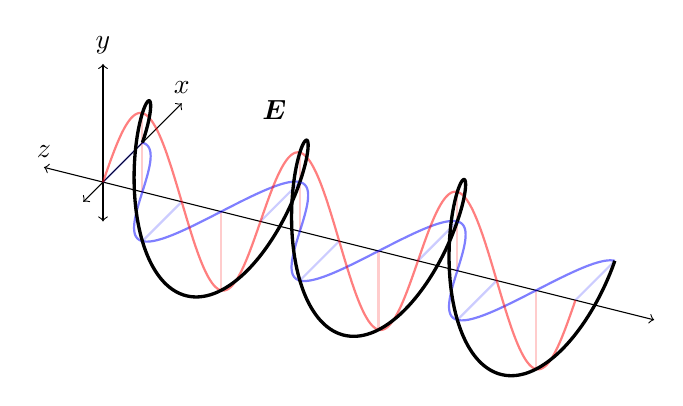
\begin{tikzpicture}[x={(0.5cm,.5cm)}, z={(1cm,-.25cm)}]

\draw[<->] (2,0,0) node[above] {$x$} -- (-0.5,0,0);
\draw[<->] (0,-0.5,0) -- (0,1.5,0) node[above] {$y$};
\draw[<->] (0,0,7) -- (0,0,-0.75) node[above] {$z$};

\tikzset{%
    xyz path/.style args={\x=#1; \y=#2; \z=#3; (#4)}{
        insert path={
            \foreach \step [evaluate={\x=#1; \y=#2; \z=#3;}] in {#4}{   
                -- (\x, \y, \z) } 
        }
    },
    cosine path/.style args={#1:#2}{
        xyz path={\x=cos(\step/2); \y=0; \z=\step/360; (#1, 5, ..., #2)},
        insert path={ coordinate (cosine path end) }
    },
    sine path/.style args={#1:#2}{
        xyz path={\x=0; \y=sin(\step/2); \z=\step/360; (#1, 5, ..., #2)},
        insert path={ coordinate (sine path end) }
    },
    spiral path/.style args={#1:#2}{
        xyz path={\x=cos(\step/2); \y=sin(\step/2); \z=\step/360; (#1, 5, ..., #2)},
        insert path={ coordinate (spiral path end) }
    }
}

\def\lastangle{720}
\def\cycles{2}

\foreach \z in {0.5,1.5,...,6} {
    \draw[-, help lines, thick, red, opacity=0.2] (0,0,\z) -- (0,{sin(deg(pi*\z))},\z);
}
\foreach \z in {0,1,...,6} {
    \draw[-, help lines, thick, blue, opacity=0.2] (0,0,\z) -- ({cos(deg(pi*\z))},0,\z);
}
\foreach \z in {0,0.02,...,6} {
    %\draw[-, help lines, opacity=0.35] (0,0,\z) -- ({cos(deg(pi*\z))},{sin(deg(pi*\z))},\z);
}

\foreach \cycle in {0,1,...,\cycles}{
    \tikzset{shift={(0, 0, 2*\cycle)}}
    \ifnum\cycle=\cycles
        \let\endangle=\lastangle
    \else
        \def\endangle{720}
    \fi
    \draw [blue, thick, opacity=0.5] (1, 0, 0) [cosine path={0:\endangle}];
    \draw [red, thick, opacity=0.5] (0, 0, 0) [sine path={0:\endangle}];
    \draw [black, very thick] (1, 0, 0) [spiral path={0:\endangle}];
}
\node[above right] at (0.8,0.65,1.5) {$\bm{E}$};

\tikzset{shift={(0,0,\cycles+\lastangle/360)}}

\end{tikzpicture}

\end{document}       